\documentclass[12pt,a4paper]{report}
\usepackage[utf8]{inputenc}
\usepackage[english,russian]{babel}
\usepackage{indentfirst}
\usepackage{pdfpages}
\usepackage{titlesec}
\usepackage{listings}

% Вставка картинки
\usepackage{graphicx}
\graphicspath{{schemes/}}
\DeclareGraphicsExtensions{.pdf,.png,.jpg}

\usepackage[14pt]{extsizes}

\newcommand{\hsp}{\hspace{20pt}}
\titleformat{\chapter}[hang]{\large\bfseries}{\thechapter{. }}{0pt}{\large\bfseries}
\titlelabel{hlabel-formati}
\titlespacing{\chapter}{42pt}{-20pt}{12pt}
\titleformat{\section}[hang]{\large\bfseries}{\thesection{. }}{0pt}{\large\bfseries}
\titlespacing{\section}{42pt}{12pt}{5pt plus 5pt}

% Отступ абзаца
\usepackage{indentfirst}
\setlength{\parindent}{1.5cm}

% Межстрочный интервал
\usepackage{setspace}
\onehalfspacing % интервал 1.5

\usepackage[left=3cm, right=1cm, top=2cm, bottom=2cm]{geometry}

\begin{document}
% Титульник
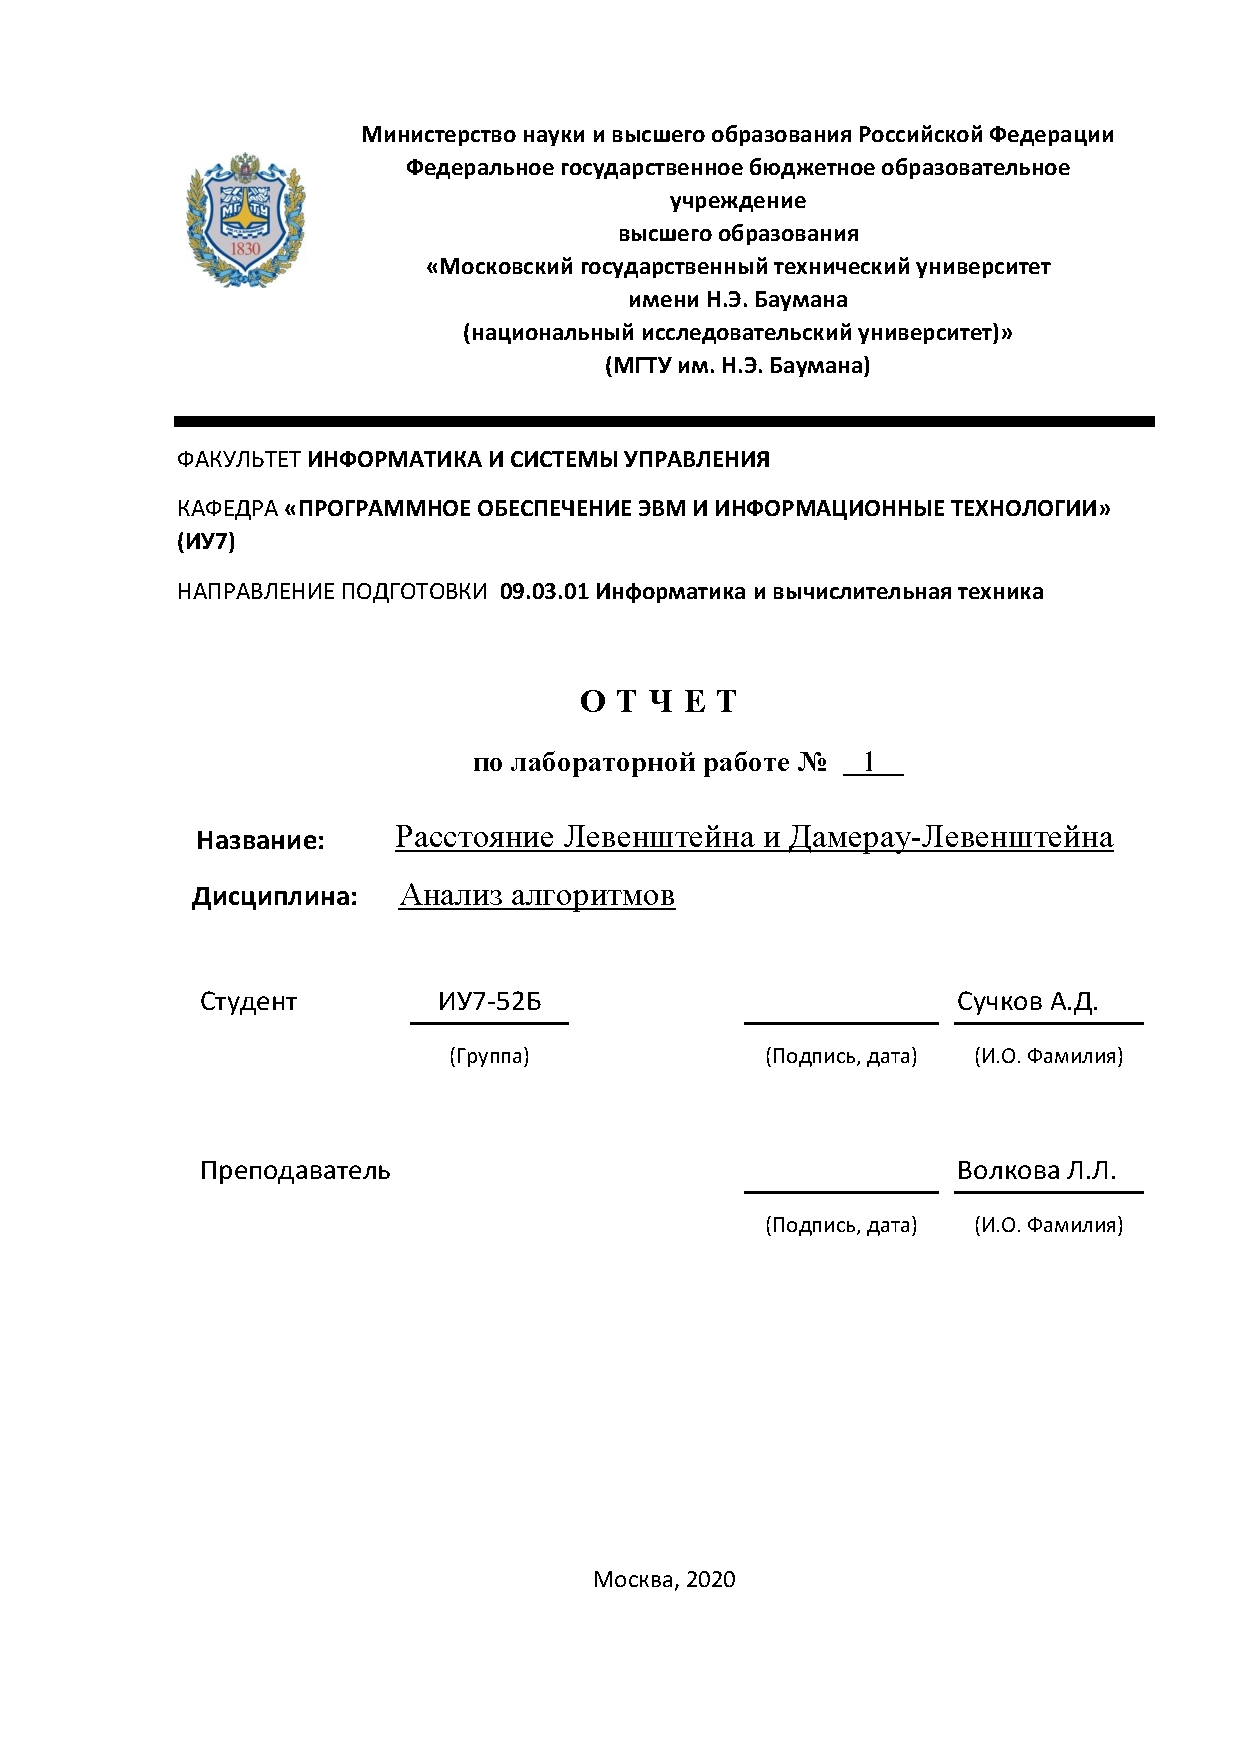
\includepdf[pages=1]{Suchkov_titul.pdf}
% Оглавление
\tableofcontents

\newpage
\chapter*{Введение}
\addcontentsline{toc}{chapter}{Введение}
\textbf{Расстояние Левенштейна} - это минимальное количество редакторских операций, которые необходимы 
для превращения одной строки в другую \cite{lev_info}. Впервые задачу поставил в 1925 году советский математик Владимир 
Левенштейн при изучении последовательностей 0 - 1, впоследствии более общую задачу для произвольного 
алфавита связали с его именем.\\

Существуют следующие редакторские операции:
\begin{itemize}
    \item вставка символа;
    \item удаление символа;
    \item замена символа.
\end{itemize} 

Расстояние Дамерау-Левенштейна включает также операцию перестановки 2 символов (или транспозицию).\\

Расстояние Левенштейна и его обобщения активно применяются для исправления ошибок в слове (в поисковых
 системах, базах данных, при вводе текста, при автоматическом распознавании отсканированного текста ил
и речи), а также, к примеру, в биоинформатике для сравнения генов, хромосом и белков.

\newpage
\chapter{Аналитическая часть}
Цель данной лабораторной работы заключается в реализации и последующем сравнении алгоритмов поиска 
расстояний Левенштейна и Дамерау-Левенштейна.\\

Для начала можно выделить следующие задачи лабораторной работы:
\begin{itemize}
    \item математически описать расстояние Левенштейна и Домерау-Левенштейна;
    \item описать и реализовать алгоритмы поиска расстояний;
    \item замерить процессорное время работы алгоритмов при различных размерах строк;
    \item оценить наибольшую затрачиваемую память для каждого из алгоритмов;
    \item провести сравнительный анализ алгоритмов на основании проведённых экспериментов; 
\end{itemize}

Поиск расстояний несёт в себе задачу нахождения такой последовательности операций, применение которых 
даст в результате минимальный суммарный штраф.\\

Существуют следующие штрафы:
\begin{itemize}
    \item вставка (I, от англ. insert) - 1;
    \item замена (R, от англ. replace) - 1;
    \item удаление (D, от англ. delete) - 1;
    \item совпадение (M, от англ. match) - 0;
    \item транспозиция (T, от англ. transposition) - 1.
\end{itemize}

Данная проблема решается использованием рекуррентной формулы вычисления расстояний. Пусть D(S1[1..i], 
S2[1..j]) - расстояние Левенштейна для подстроки S1 и S2 с длинами i и j соответственно.\\\\

Тогда, формула для вычисления D имеет следующий вид:

\begin{displaymath}
    D(i,j) = \left\{ 
        \begin{array}{ll}
            j, & \textrm{если i = 0} \\
            i, & \textrm{если j = 0} \\
            min(D(S1[1..i], S2[1..j-1]) + 1,\\
                D(S1[1..i-1], S2[1..j]) + 1,\\
                D(S1[1..i-1], S2[1..j-1] + \left \{ 
                \begin{array}{ll}
                    0, \textrm{если S1[i] = S2[j]} \\ 
                    1, \textrm{иначе}
                \end{array} \right.
            )
        \end{array} \right.
\end{displaymath} \\

Аналогично и для Дамерау-Левенштейна:

\begin{displaymath}
    D(i, j) = \left\{
        \begin{array}{ll}
            j, \textrm{если i = 0} \\
            i, \textrm{если j = 0} \\
            min(D(S1[1..i], S2[1..j-1]) + 1,\\
                D(S1[1..i-1], S2[1..j]) + 1,\\
                D(S1[1..i-1], S2[1..j-1] + \left \{ 
                \begin{array}{ll}
                    0, \textrm{если S1[i] = S2[j]} \\ 
                    1, \textrm{иначе}
                \end{array} \right.
            , \\
                \left \{ \begin{array}{ll}
                    D(S1[1..i-2], S2[1..j-2]) + 1 \textrm{, если} \left \{ 
                    \begin{array}{ll}
                        i > 1, j > 1 \\
                        S1[i] = S2[j-1] \\
                        S1[i-1] = S2[j]
                    \end{array} \right. \\
                    +\infty, \textrm{иначе}
                \end{array} \right. 
            )
    \end{array} \right.
\end{displaymath}

\newpage
\chapter{Конструкторская часть}

Рассмотрим алгоритмы поиска расстояний Левенштейна и Дамерау-Левенштейна для строк S1 и S2 с длинами 
l1 и l2 соответственно.

\section{Расстояние Левенштейна, рекурсивный метод}

В методе используется рекурсивная формула нахождения D(S1[1..i], S2[1..j]), реализовать это можно 
с помощью рекурсивной функции. Функция будет принимать в качестве входных данных строки S1 и S2, а 
также их длины i и j соответственно. Метод основан на последующем вызове той же функции для тех же 
строк, но для длин (i-1, j-1), (i-1, j), (i, j-1), где возвращается минимальное из этих значений. 
Схема на рис. 2.1.

\section{Расстояние Левенштейна, матричный метод}

Данный матричный метод основан на использовании рекуррентной формулы. В начале работы создаётся 
целочисленная матрица с размерами (l1 + 1) на (l2 + 1), затем заполняются первый столбец и первая 
строка, которые являются базой для рекуррентной формулы. Матрица заполняется построчно, в каждой 
ячейке [i][j] матрицы записывается значение D(S1[1..i-1], S2[1..j-1]). В том случае, когда i=1 и 
j=1 будет значить, что строки пусты. Итоговым результатом является значение в нижней правой ячейке
 матрицы, т.е. в ячейке с индексом [l1 + 1][l2 + 1]. Схема на рис. 2.2.

\section{Расстояние Левенштейна, рекурсивный метод с заполнением матрицы}

В данном методе создаётся матрица размерами (l1 + 1)x(l2 + 1), все ячеки которой изначально заполнены 
значением бесконечности. В каждой клетке [i][j] этой матрицы будет записано значение D(s1[1..i-1], s2[1..j-1]).

Рекурсивная функция получает матрицу, индексы i, j положения в ней и две строки. Алгоритм начинает свою 
работу с ячейки [1][1], которая заполняется значением 0. Из положения [i][j] рассматривается переход в 
соседние ячейки [i + 1][j + 1], [i + 1][j], [i][j + 1]. В случае, если соседняя ячейка расположена в 
пределах матрицы и расстояние R при переходе из данной ячейки меньше ныне хранимого в ней значения, то 
значение соседней ячейки меняется на R, после чего функция запускается уже для соседней ячейки. После 
завершения работы всех функций, расстояние Левенштейна расположено в ячейке [l1 + 1][l2 + 1]. Схема на
рис. 2.3.

\section{Расстояние Дамерау-Левенштейна, матричный метод}

Метод является модифицированным методом подсчёта расстояния Левенштейна матричным методом. В матрице
для ячейки [i][j], где i > 2 и j > 2, учитывается также вариант перехода из клетки [i-2][j-2], в 
случае когда S1[i] = S2[j-1] и S1[i-1] = S[j]. Результатом всё также будет правое нижнее значение
ячейки [l1 + 1][l2 + 1]. Схема на рис 2.4.

\section{Требования к программе}

Для дальнейшего тестирования программы необходимо обеспечить консольный ввод двух строк, а также
обеспечить выбор алгоритма поиска. На выходе должны получить редакционное расстояние и, если 
использовался один из матричных методов, программа должна выводить саму матрицу подсчёта.\\

Также необходимо реализовать функцию подсчёта процессорного времени, которое могут затрачивать 
функции поиска.

\section{Тесты}

Для детального тестирования программы, можно выделить несколько случаев поступаемых данных:
\begin{itemize}
    \item равные (одинаковые) строки;
    \item одна из строк пуста;
    \item две строки пусты;
    \item проверка транспозиции (для Дамерау-Левенштейна).
\end{itemize}

\begin{figure}[h]
\center{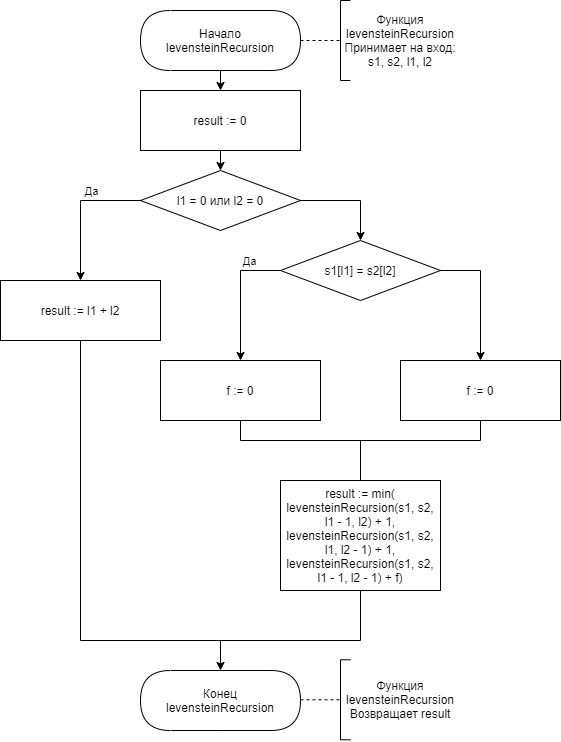
\includegraphics[scale=1.2]{scheme_levensteinRecursion}}
\caption{Расстояние Левенштейна, рекурсивный метод}
\label{fig:image}
\end{figure}

\begin{figure}[h]
\center{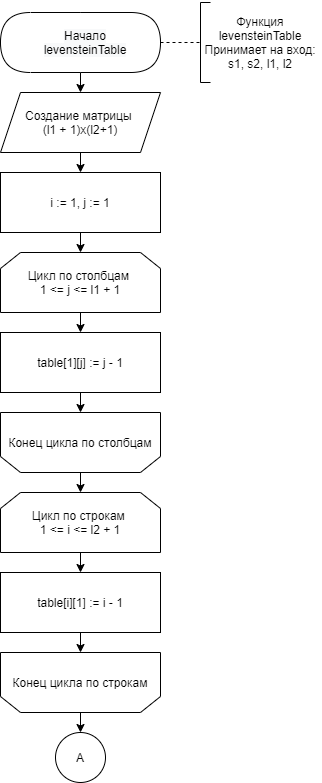
\includegraphics[scale=1.2]{scheme_levensteinTable_1}}
\caption{Расстояние Левенштейна, матричный метод, часть 1}
\label{fig:image}
\end{figure}

\begin{figure}[h]
\center{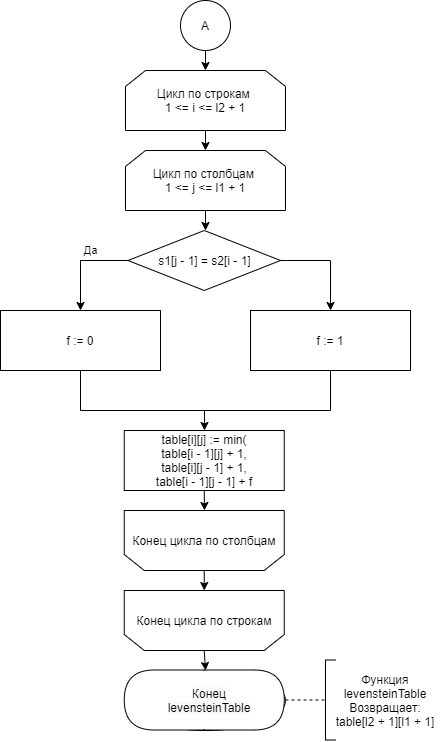
\includegraphics[scale=1.2]{scheme_levensteinTable_2}}
\caption{Расстояние Левенштейна, матричный метод, часть 2}
\label{fig:image}
\end{figure}

\begin{figure}[h]
\center{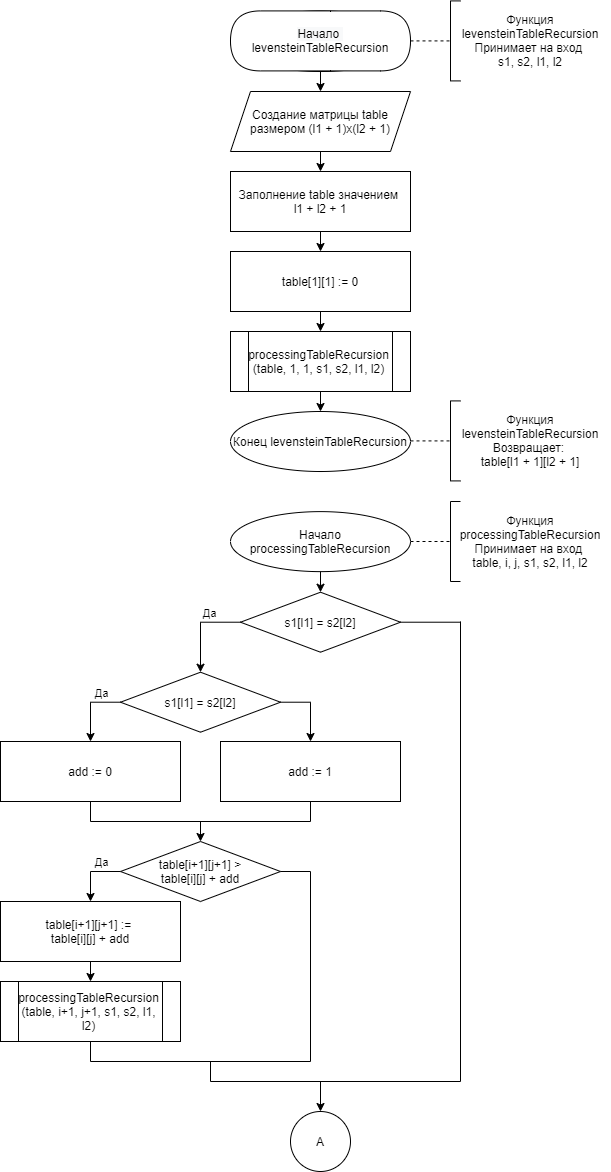
\includegraphics[scale=1]{scheme_levensteinTableRecursion_1}}
\caption{Расстояние Левенштейна, рекурсивный метод с заполнением матрицы, часть 1}
\label{fig:image}
\end{figure}

\begin{figure}[h]
\center{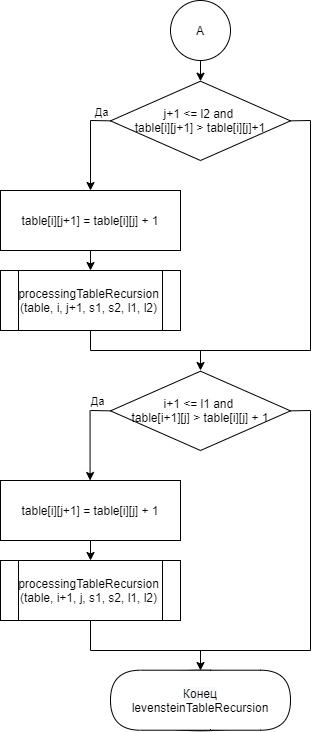
\includegraphics[scale=1.2]{scheme_levensteinTableRecursion_2}}
\caption{Расстояние Левенштейна, рекурсивный метод с заполнением матрицы, часть 2}
\label{fig:image}
\end{figure}

\begin{figure}[h]
\center{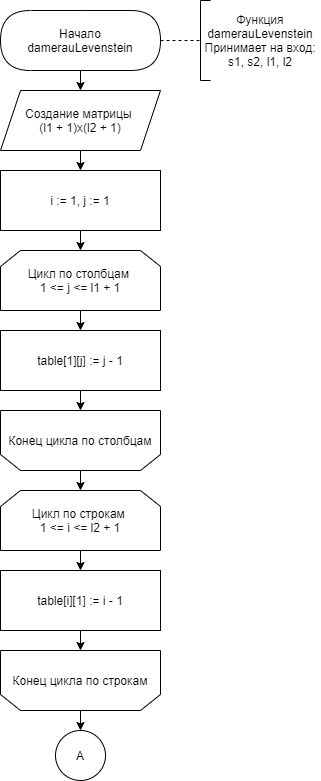
\includegraphics[scale=1.2]{scheme_damerauLevenstein_1}}
\caption{Расстояние Дамерау-Левенштейна, матричный метод, часть 1}
\label{fig:image}
\end{figure}

\begin{figure}[h]
\center{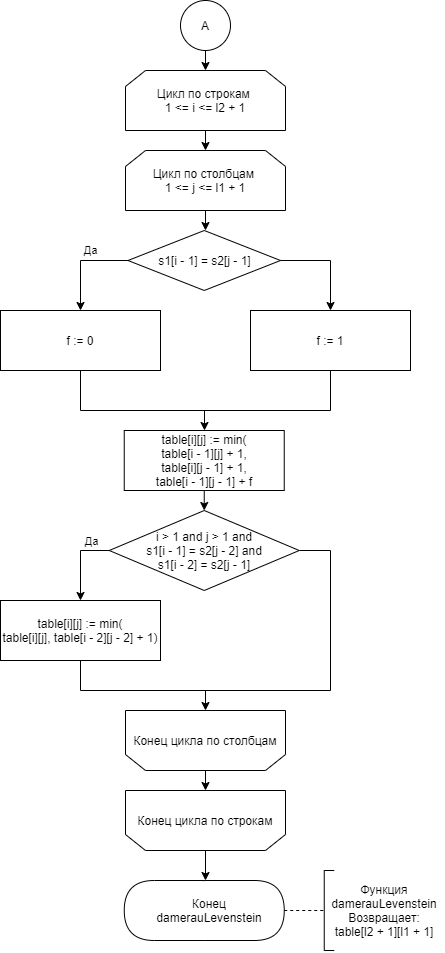
\includegraphics[scale=1]{scheme_damerauLevenstein_2}}
\caption{Расстояние Дамерау-Левенштейна, матричный метод, часть 2}
\label{fig:image}
\end{figure}

\newpage
\chapter{Технологическая часть}

\section{Выбор языка программирования}

В качестве языка программирования было решено выбрать Python 3, так как уже имеется опыт работы с 
библиотеками и инструмантами языка, которые позволяют реализовать и провести исследования алгоритмов
подсчёта расстояния.

\section{Листинг кода реализованных алгоритмов}

Далее с листинга 3.1 по 3.4 приведены реализации алгоритмов подсчёта расстояния Левенштейна и Дамерау-Левенштейна.

\textrm{Листинг 3.1: расстояние Левенштейна, рекурсивный метод}
\begin{lstlisting}[frame=single, numbers=left]
def levensteinRecursion(s1, s2):
    if (s1 == "" or s2 == ""):
        return len(s1) + len(s2)

    if (s1[-1] == s2[-1]): 
        f = 0 
    else: 
        f = 1

    return min(levensteinRecursion(s1, s2[:-1]) + 1,
               levensteinRecursion(s1[:-1], s2) + 1,
               levensteinRecursion(s1[:-1], s2[:-1]) + f)
\end{lstlisting}


\textrm{Листинг 3.2: расстояние Левенштейна, матричный метод}
\begin{lstlisting}[frame=single, numbers=left]
def levensteinTable(s1, s2, isPrint):
    lenI = len(s1) + 1
    lenJ = len(s2) + 1

    table = [[i + j for j in range(lenJ)] 
                    for i in range(lenI)]

    for i in range(1, lenI):
        for j in range(1, lenJ):
            if (s1[i - 1] == s2[j - 1]):
                f = 0 
            else:
                f = 1
            table[i][j] = min(table[i - 1][j] + 1,
                              table[i][j - 1] + 1,
                              table[i - 1][j - 1] + f)
    if (isPrint):
        tablePrint(table)
    
    return table[-1][-1]
\end{lstlisting}

\textrm{Листинг 3.3: расстояние Левенштейна, рекурсивный метод с заполнением матрицы}
\begin{lstlisting}[frame=single, numbers=left]
def processingTableRecursion(table, i, j, s1, s2):
    if (i + 1 < len(table)) and (j + 1 < len(table[0])):
        if s1[j] == s2[i]:
            add = 0
        else:
            add = 1 
        
        if table[i + 1][j + 1] > table[i][j] + add:
            table[i + 1][j + 1] = table[i][j] + add
            processingTableRecursion(table, i + 1, 
                                     j + 1, s1, s2)
    
    if (j + 1 < len(table[0])) and 
       (table[i][j + 1] > table[i][j] + 1):
        table[i][j + 1] = table[i][j] + 1
        processingTableRecursion(table, i, j + 1, s1, s2)

    if (i + 1 < len(table)) and 
       (table[i + 1][j] > table[i][j] + 1):
        table[i + 1][j] = table[i][j] + 1
        processingTableRecursion(table, i + 1, j, s1, s2)
    
def levensteinTableRecursion(s1, s2, isPrint):
    lenI = len(s1) + 1
    lenJ = len(s2) + 1

    maxLen = max(len(s1), len(s2)) + 1

    table = [[maxLen] * lenI for i in range(lenJ)]
    table[0][0] = 0

    processingTableRecursion(table, 0, 0, s1, s2)

    if isPrint:
        tablePrint(table)
    
    return table[-1][-1]
\end{lstlisting}

\textrm{Листинг 3.4: расстояние Дамерау-Левенштейна, матричный метод}
\begin{lstlisting}[frame=single, numbers=left]
def damerauLevenstein(s1, s2, isPrint):
    lenI = len(s1) + 1
    lenJ = len(s2) + 1
    
    table = [[i + j for j in range(lenJ)] 
                    for i in range(lenI)]

    for i in range(1, lenI):
        for j in range(1, lenJ):
            if (s1[i - 1] == s2[j - 1]):
                f = 0
            else:
                f = 1
            
            table[i][j] = min(table[i - 1][j] + 1,
                              table[i][j - 1] + 1,
                              table[i - 1][j - 1] + f)
            

            if (i > 1 and j > 1) and 
               (s1[i - 1] == s2[j - 2]) and 
               (s1[i - 2] == s2[j - 1]):
                table[i][j] = min(table[i][j], 
                table[i - 2][j - 2] + 1)
        
    if isPrint:
        tablePrint(table)
    
    return table[-1][-1]
\end{lstlisting}

\section{Результаты тестирования}

Для модульного тестирования реализованных алгоритмов, были написаны специальные функции с наборами тестов:

\textrm{Листинг 3.5: Модульные тесты}
\begin{lstlisting}[frame=single, numbers=left]
def doUnitTest(testArray, testName, levFunction, isTable):
    for i in range(len(testArray)):
        if (isTable):
            result = levFunction(testArray[i][0], 
                                 testArray[i][1], False)
        else:
            result = levFunction(testArray[i][0], 
                                 testArray[i][1])

        if (result == testArray[i][2]):
            print(testName, "test", i, "succesfully")
        else:
            print(testName, "test", i, "failure")
            return False
    
    return True


def unitTests(levFunction, isTable):
    # Tests with empty string
    test_empty = [["f", "f", 0], 
                  ["f", "", 1], 
                  ["", "f", 1]]
    # Test with match
    test_match = [["asd", "asd", 0], 
                  ["f", "f", 0], 
                  ["F", "f", 1]]
    # Others tests
    test_others = [["a", "s", 1], 
                   ["asd", "bsf", 2], 
                   ["asd", "as", 1], 
                   ["a", "adws", 3]]

    if doUnitTest(test_empty, "Empty", 
                  levFunction, isTable):
        print()
        if doUnitTest(test_match, "Match", 
                      levFunction, isTable):
            print()
            if doUnitTest(test_others, "Others", 
                          levFunction, isTable):
                print("\n>>>All tests done!\n")
\end{lstlisting}

Все тесты прошли успешно

\section{Оценка затрачиваемой памяти}

Для подсчёта наибольшей занимаемой памяти $M_{max}$ каждого алгоритма, пусть для удобства строки 
s1 и s2 имеют одиноковую длину l.

\underline{Расстояние Левенштейна, рекурсивный метод}

Функция будет запрашивать память при каждом вызове. Функция принимает на вход две строки и каждый раз 
подсчитывает и хранит два размера этих строк. Максимальная глубина рекурсии = l + l.

$M_{max}$ = (l + l) * (2l * sizeof(char) + 2 * sizeof(int)) = 2l * (2l + 32) = 4$l^2$ + 64l байт. \\

\underline{Расстояние Левенштейна, матричный метод}

В данном алгоритме память тратится на матрицу и две строки.

$M_{max}$ = (l + 1) * (l + 1) * sizeof(int) + (l + l) * sizeof(char) = (l + 1) * (l + 1) * 16 + 2l = 
16$l^2$ + 2 * 17l + 16 байт. \\

\underline{Расстояние Левенштейна, рекурсивный метод с заполнением матрицы}

Память тратится на матрицу и при каждом вызове функции. Максимальная глубина рекурсии = l + l.

$M_{max}$ = (l + 1) * (l + 1) * sizeof(int) + (l + l) * (2l * sizeof(char) + 2 * sizeof(int)) = ($l^2$ + 
2l + 1) * 16 + 2l * (2l + 32) = 20$l^2$ + 96l + 16 байт. \\

\underline{Расстояние Дамерау-Левенштейна, матричный метод}

Память, также как и в матричном алгоритме Левенштейна тратится на матрицу и две строки.

$M_{max}$ = 16 * $l^2$ + 2 * 17l + 16 байт. \\

\section{Оценка затрачиваемого времени}

Для замера процессорного времени выполнения алгоритмов используется библиотека time \cite{time_bib}. В листинге 3.6 
приведена функция генерации случайной строки заданной длины. В листинге 3.7 приведены функции, с 
помощью которых производились замеры.

\newpage
\textrm{Листинг 3.6: Функция генерации строки заданной длинны с произвольными символами}
\begin{lstlisting}[frame=single, numbers=left]
def takeRandomString(size):
    return ''.join(random.choice(string.ascii_letters) 
                   for _ in range(size))
\end{lstlisting}

\textrm{Листинг 3.7: Функции для замера времени}
\begin{lstlisting}[frame=single, numbers=left]
def doTimeTestsRecursion(levFunc, iterations, strLength):
    t1 = process_time()

    for _ in range(iterations):
        s1 = takeRandomString(strLength)
        s2 = takeRandomString(strLength)
        levFunc(s1, s2)

    t2 = process_time()

    return (t2 - t1) / iterations


def doTimeTestsTable(levFunc, iterations, strLength):
    t1 = process_time()

    for _ in range(iterations):
        s1 = takeRandomString(strLength)
        s2 = takeRandomString(strLength)
        levFunc(s1, s2, False)

    t2 = process_time()

    return (t2 - t1) / iterations

def timeTests(levFunction, isTable, isRecursion):
    lengthsArray = [1, 3, 10, 20, 100, 1000]
    iterations   = [100000, 10000, 100, 200, 100, 10]

    if (isRecursion):
        lastIndex = 3
    else:
        lastIndex = len(lengthsArray)

    for i in range(lastIndex):
        if (isTable):
            timeResult = doTimeTestsTable(levFunction, 
                                          iterations[i], 
                                          lengthsArray[i])
        else:
            timeResult = doTimeTestsRecursion(levFunction, 
                iterations[i], lengthsArray[i])
        
        print("For length =", lengthsArray[i], 
              "\ttime =", timeResult)
\end{lstlisting}


\newpage
\chapter{Исследовательская часть}

Измерения процессорного времени проводятся при одинаковых длинах строк s1 и s2, при этом всём 
содержание наполняется случайно генерируемыми символами. Эксперименты по замеру времени проводились 
при длинах 1, 3, 7, 20, 100, 1000.

\section{Результаты экспериментов}

Проведя измерения процессорного времени выполнения реализованных алгоритмов, можно составить таблицу 4.1

\begin{table}
\caption{Результаты замеров процессорного времени в секундах}
\label{tabular:timesandtenses}
\begin{center}
\begin{tabular}{ | l | l | l | l | l | l | l |}
\hline
Название метода       & 1         & 3         & 7         & 20        & 100       & 1000  \\ \hline
Лев. рекурсия         & 3.8 *     & 2 *       & 6 *       & --        & --        & --    \\ 
                      & $10^{-6}$ & $10^{-4}$ & $10^{-1}$ &           &           &       \\ \hline
Лев. матрица          & 7 *       & 2.2 *     & 1.3 *     & 4.7 *     & 9 *       & 1.321 \\
                      & $10^{-6}$ & $10^{-5}$ & $10^{-4}$ & $10^{-4}$ & $10^{-3}$ &       \\ \hline
Лев. рекурсия-матрица & 1 *       & 4 *       & 2 *       & 2.5       & --        & --    \\
                      & $10^{-5}$ & $10^{-5}$ & $10^{-4}$ & $10^{-3}$ &           &       \\ \hline
Дамерау-Левенштейна   & 7.5 *     & 2.7 *     & 1.5 *     & 6 *       & 0.012     & 1.725 \\
                      & $10^{-6}$ & $10^{-5}$ & $10^{-4}$ & $10^{-4}$ &           &       \\ 
\hline
\end{tabular}
\end{center}
\end{table}

\section{Сравнительный анализ}

Анализируя полученные результаты можно сказать, можно выделить несколько утверждений:

\begin{itemize}
    \item наименее время затратным является алгоритм, использующий матрицу;
    \item рекурсивный алгоритм с заполнением матрицы демонстрирует значительно низкую скорость роста времени по сравнению с рекурсивным алгоритмом;
    \item алгоритм поиска расстояний Левенштейна и Дамерау-Левенштейна с помощью матриц показывают схожую скорость роста времени, однако первый алгоритм несколько быстрее.
\end{itemize}

\newpage
\chapter*{Заключение}
\addcontentsline{toc}{chapter}{Заключение}

В ходе выполнения лабораторной работы были решены все задачи и достигнута цель, а именно реализация и 
сравнение алгоритмов поиска расстояний Левенштейна и Дамерау-Левенштейна. Были изучены и описаны понятия 
расстояний Левенштейна и Дамерау-Левенштейна, а также были описаны и реализованы алгоритмы поиска 
расстояния, проведены замеры процессорного времени работы каждого алгоритма при различных строках. Была 
произведена оценка наибольшей занимаемой памяти. Проведён сравнительный анализ алгоритмов.

\renewcommand\bibname{Список литературы}
\addcontentsline{toc}{chapter}{Список литературы}
\makeatletter % список литературы
\def\@biblabel#1{#1. }
\makeatother
\begin{thebibliography}{2}
    \bibitem{lev_info} Мосалев П.М. Обзор методов нечеткого поиска текстовой информации // Вестник МГУП. 2016. №2. (дата обращения 23.09.2020)
    \bibitem{time_bib} Документация на официальном сайте Python про библиотеку time [Электронный ресурс]. Режим доступа: https://docs.python.org/3/library/time.html (дата обращения 23.09.2020)
\end{thebibliography}

\end{document}

